\subsection{Bestimmung der Ankerinduktivität}


\begin{figure}[H]
    \centering
    % 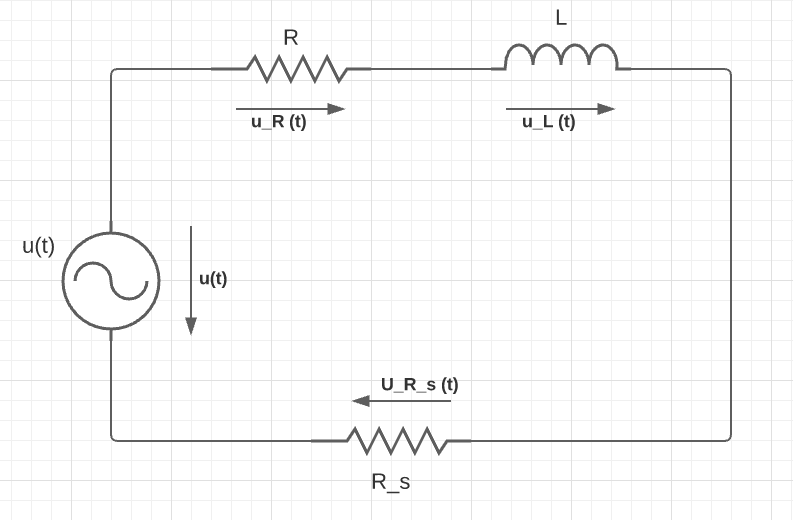
\includegraphics[width=1\textwidth]{schaltplan.png}
    \caption{Mess-Schaltung Ankerinduktivität}
    \label{fig:PlotAufgabe1}
   \end{figure}


\begin{equation} \label{eq211}
    \begin{split}
        u(t)&=u_R(t) + u_L(t)\\
        u(t)&=R \cdot i(t) + L \frac{d i(t)}{dt}\\
        u(t)&= (R+R_s) \cdot i(t) + L \frac{d i(t)}{dt}
    \end{split}
\end{equation}

